\documentclass{fieldpractice-geo}
% 添加目录页的内容,\title为标题,\faculty为学院,\name为姓名,\xuehao为学号,\grade为年级,\class为班级
\title{地理学野外实习报告模板}
\faculty{地理科学学院}
\name{XX}
\xuehao{10XX39034XX}
\grade{20XX}
\class{XX班}

\begin{document}
	\maketitle

\section{正文格式}
报告正文格式要求:
\begin{enumerate}
	\item 报告中凡是数字、英文与符号均用Times New Roman字体,中文用宋体,字号为小四,1.25倍行间距
	\item 报告中出现的图、表须有图名、表名,图名放在图下方,表名放在表上方,图名与表名及表中文字均用五号字,如下所示。表中文字字号用小五。图、表均居中。
	\item 手绘剖面图须有比例尺、剖面方位等基本图件要素(若为野外手绘剖面,可扫描后以图片的方式插入报告中,也可将最终的报告打印后,在预留的地方根据野外记录重新用铅笔绘制)
	\item 按在报告中出现的先后顺序给图、表编号,并以序号在报告文稿中引用图、表,如:××××地区石炭系地层以竹叶状灰岩为主(图\ref{fig:XXXX地区石炭系竹叶状灰岩})××××地区地层(表\ref{tab:××××地区地层})
	\item 图片在报告中的合适位置以“嵌入”方式插入并居中显示,\textcolor{blue}{图片需成比例缩放,不可随意改变水平比例与垂直比例,使得地质体比例失调。}
	\item 报告中地层需标注正确,并合理使用上、下标,如\textcolor{blue}{下三叠统($T_1$,而不是T1)}
	\item \textcolor{blue}{报告杜绝错别字!}
	\item \textcolor{blue}{报告左侧装订(不需要塑料文件夹等装饰)}
\end{enumerate}
\begin{figure}[ht]
	\centering
	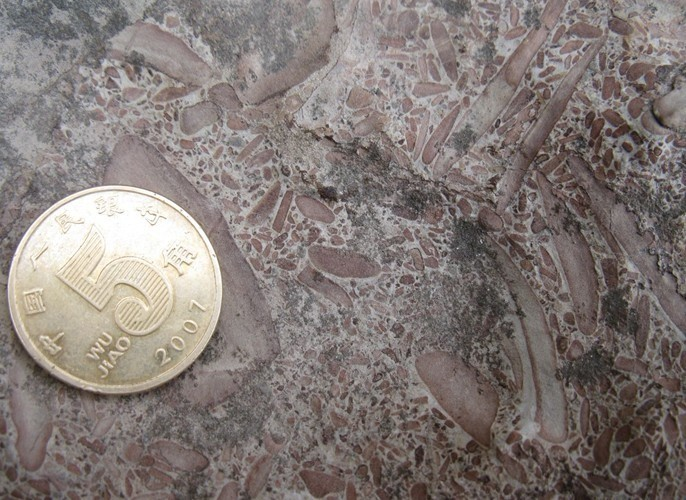
\includegraphics[width=0.6\textwidth]{figures/XXXX地区石炭系竹叶状灰岩.jpg}
	\caption{XXXX地区石炭系竹叶状灰岩}
	\label{fig:XXXX地区石炭系竹叶状灰岩}
\end{figure}
\begin{table}[htbp]
	\centering
	\caption{××××地区地层}
	\begin{tabular}{ccccc}
		\toprule
		1 &  1     & 1      &  1     & 1 \\
		\midrule
		1 & 1      & 1      &  1     & 1 \\
		1 & 1      & 1      &  1     & 1 \\
		1 & 1      & 1      &  1     & 1 \\
		\bottomrule
	\end{tabular}%
	\label{tab:××××地区地层}%
\end{table}%

参考文献格式:

 \textcolor{red}{该模板使用bibtex进行参考文献管理,引用格式为unsrt,引用类型如下:}
\begin{itemize}
	\item 按参考文献在报告中出现的先后顺序依次列出,报告中引用该参考文献的序号:
	××××地区中生代时期主要为海相环境\cite{地质学基础}
	\item article
	\begin{figure}[H]
		\centering
		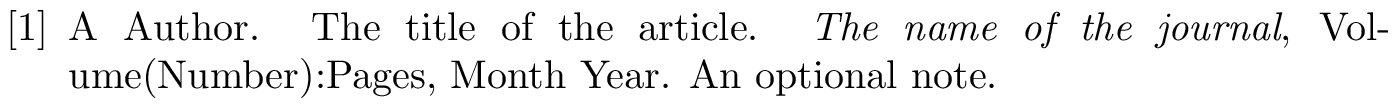
\includegraphics[width=1\textwidth]{example-figures/article.png}
		\caption*{}
	\end{figure}
	\item book 
	\begin{figure}[H]
	\centering
	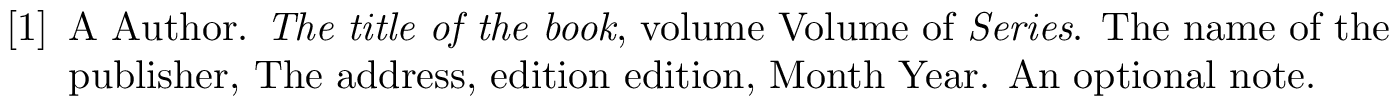
\includegraphics[width=1\textwidth]{example-figures/book.png}
	\caption*{}
	\end{figure}
	\item booklet
	\begin{figure}[H]
	\centering
	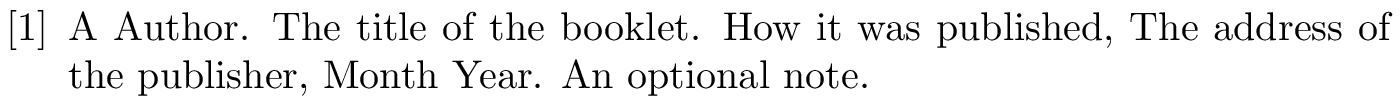
\includegraphics[width=1\textwidth]{example-figures/booklet.png}
	\caption*{}
	\end{figure}
	\item inbook
	\begin{figure}[H]
		\centering
		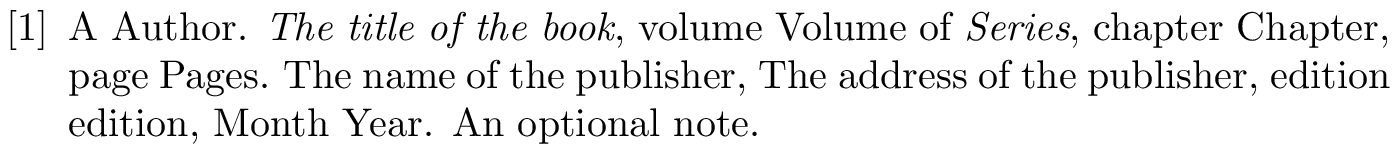
\includegraphics[width=1\textwidth]{example-figures/inbook.png}
		\caption*{}
	\end{figure}
	\item incollection
	\begin{figure}[H]
		\centering
		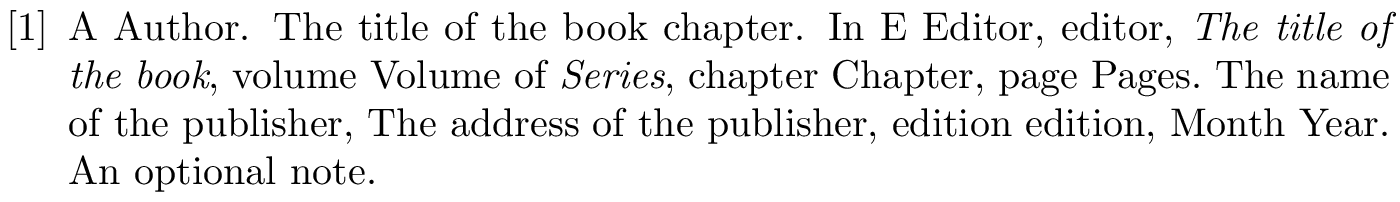
\includegraphics[width=1\textwidth]{example-figures/incollection.png}
		\caption*{}
	\end{figure}
	\item inproceedings
	\begin{figure}[H]
		\centering
		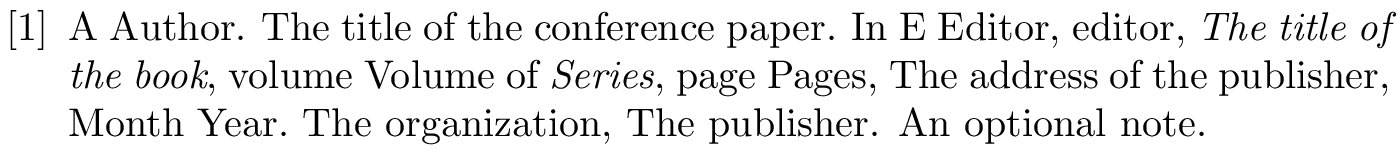
\includegraphics[width=1\textwidth]{example-figures/inproceedings.png}
		\caption*{}
	\end{figure}
	\item manual
	\begin{figure}[H]
		\centering
		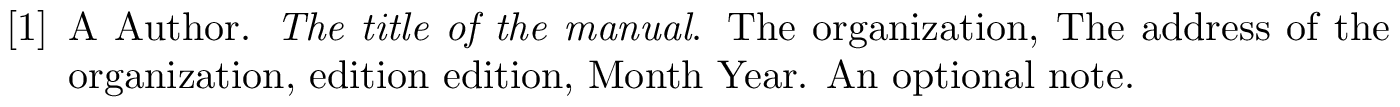
\includegraphics[width=1\textwidth]{example-figures/manual.png}
		\caption*{}
	\end{figure}
	\item masterthesis
	\begin{figure}[H]
		\centering
		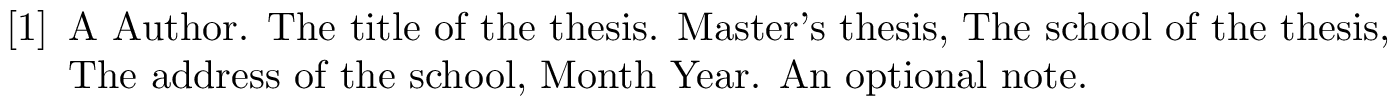
\includegraphics[width=1\textwidth]{example-figures/masterthesis.png}
		\caption*{}
	\end{figure}
	\item misc
	\begin{figure}[H]
		\centering
		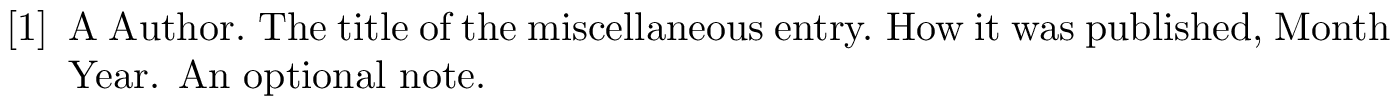
\includegraphics[width=1\textwidth]{example-figures/misc.png}
		\caption*{}
	\end{figure}
	\item phdthesis
	\begin{figure}[H]
		\centering
		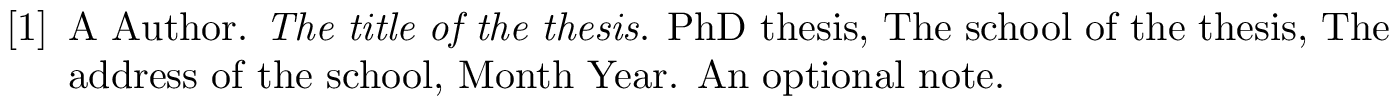
\includegraphics[width=1\textwidth]{example-figures/phdthesis.png}
		\caption*{}
	\end{figure}
	\item proceedings
	\begin{figure}[H]
		\centering
		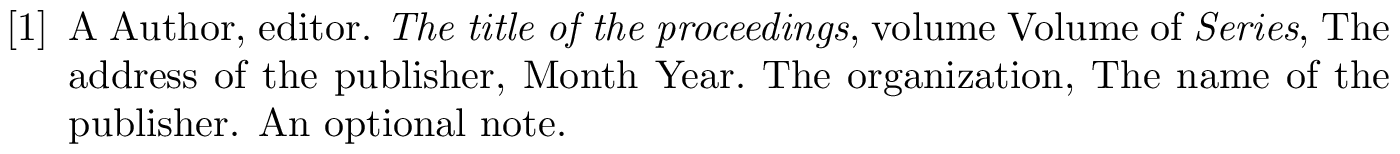
\includegraphics[width=1\textwidth]{example-figures/proceedings.png}
		\caption*{}
	\end{figure}
	\item techreport
	\begin{figure}[H]
		\centering
		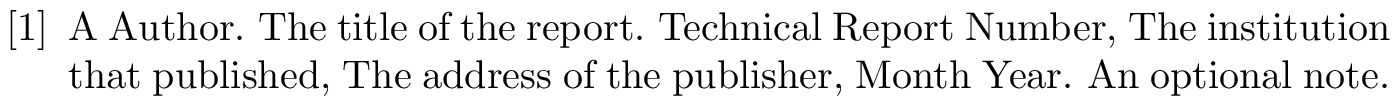
\includegraphics[width=1\textwidth]{example-figures/techreport.png}
		\caption*{}
	\end{figure}
	\item unpublished
	\begin{figure}[H]
		\centering
		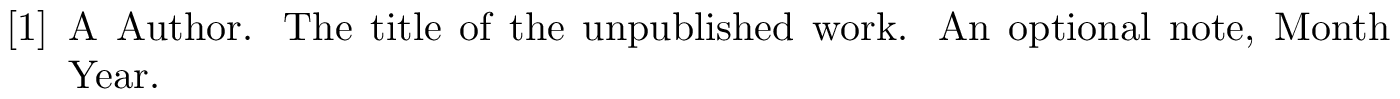
\includegraphics[width=1\textwidth]{example-figures/unpublished.png}
		\caption*{}
	\end{figure}
\end{itemize}
% Word格式要求:
% \begin{enumerate}
% 	\item 按参考文献在报告中出现的先后顺序依次列出,报告中引用该参考文献的序号:
% 	××××地区中生代时期主要为海相环境\cite{地质学基础}
% 	\item 参考文献用五号字,其中的数字、英文与符号均用Times New Roman字体,中文用宋体,如下所示
% 	\item 参考文献格式须统一格式为:
% 	全体作者(作者之间已英文逗号相隔), 参考书目或文章名称, 出版社或期刊名称, 出版年份, (期刊文章还需给出卷, 期), 页码(若引用书目,则为引用页码;若为期刊文章,则为该文章的页码)。
% \end{enumerate}
\begin{table}[htbp]
	\centering
	\caption{已加载的宏包}
	\begin{tabular}{cccc}
		\toprule
		\multicolumn{4}{c}{packages loaded} \\
		\midrule
		algorithm & algorithmicx & algpseudocode & amsfonts \\
		amsmath & amssymb & amsthm & array \\
		bigdelim & bigstrut & bm    & booktabs \\
		caption & cite  & cprotect & ctex \\
		diagbox & enumitem & fancyhdr & float \\
		fontspec & geometry & graphicx & hyperref \\
		ifthen & ifxetex & indentfirst & lipsum \\
		listings & longtable & multirow & placeins \\
		tabularx & titlesec & titletoc & tocloft \\
		ulem  & url   & xcolor & xeCJK \\
		xunicode & zhlipsum & zhnumber &  \\
		\bottomrule
	\end{tabular}%
	\label{tab:已加载的宏包}%
\end{table}%

\section{前言}
(简要介绍本次实习的目的、实习区基本情况)

\section{地层特征描述}
\subsection{火成岩}
(根据自己的野外记录包括照片,描述在苏州天平山见到的火成岩地质现象)
\subsection{沉积岩}
(介绍野外考察的地层,按从老到新的顺序介绍)
\subsubsection{}

\section{构造现象描述}
\subsection{褶皱}

\subsection{断层}

\subsection{节理}

\section{地质演化简史}
(根据以上内容,归纳、总结实习区地质演化历史)

%	控制参考文献格式
\geobibstyle
% 添加参考文献,使用bibtex管理,{}内为.bib的文件名(可以不带前缀)
\bibliography{bibliography}

\end{document}